\documentclass[11pt]{article}

\usepackage{graphicx}
\usepackage{html}


%  Set lengths for nicer output.

\setlength{\textwidth}{160mm}
\setlength{\textheight}{230mm}
\setlength{\topmargin}{-2mm}
\setlength{\oddsidemargin}{0mm}
\setlength{\evensidemargin}{0mm}
\setlength{\parindent}{0mm}
\setlength{\parskip}{\medskipamount}
\setlength{\unitlength}{1mm}

%  New private macros.

\newenvironment{squote}{\begin{quote}\small}{\end{quote}}
\newcommand{\xref}[3]{\htmladdnormallink{#1}{http://www.starlink.rl.ac.uk/cgi-bin/htxserver/#2.htx/?xref_#3}}


\begin{document}


\section{Astrometric calibration for INT Wide Field Camera images}

The Wide Field Camera instrument on the Isaac Newton Telescope 
contains four CCD chips of 2048 $\times$ 4096 pixels 
positioned roughly, but not exactly, as follows:
\begin{quote}
\begin{center}
\latexhtml{\includegraphics{ideal.eps}}{\htmladdimg{ideal.gif}}
\end{center}
\end{quote}
In order to do accurate astrometry with data obtained
from this instrument, it is necessary to correct for the 
exact orientation and position of each CCD in relation to
the others, as well as for nonlinear distortions
away from the optical axis of the focal plane introduced by
the optics of the telescope.
The nonlinear distortion is very well modelled by a radial ``pincushion''
transformation, which has the form
\begin{displaymath}
  r' = r ( 1 + D r^2 )
\end{displaymath}

The following transformations take account of both these effects
to map the pixel coordinates $(x_i, y_i)$
of CCD\#$i$ into a new pixel-like coordinate system 
$(x', y')$
of uniform scale, which is the same for all four CCDs.
The origin of this coordinate system is at pixel coordinates
$(1778, 3029)$ of CCD\#4, which is taken to be on the optical axis.
At this point, one unit of the new coordinate system is equivalent
to one pixel of the CCD\#4 system, so that the new coordinates 
are almost equivalent to CCD\#4 coordinates, although they diverge
away from the origin thanks to the nonlinear distortion.
Each unit of the new coordinates has the same size, 
which is approximately 0.333 arcsec.

The corrected coordinates $(x', y')$ are obtained from 
each set of pixel coordinates $(x_i, y_i)$
by first translating so that the origin is on the optical
axis, then rotating to the correct angle, 
then correcting for the radial distortion effect:
\begin{eqnarray*}
  x_i^{\rm shift} & = & x_i - X_i \\
  y_i^{\rm shift} & = & y_i - Y_i \\[1ex]
%
  x_i^{\rm rot}   & = & x_i^{\rm shift} \cos \theta_i 
                      - y_i^{\rm shift} \sin \theta_i  \\
  y_i^{\rm rot}   & = & x_i^{\rm shift} \sin \theta_i 
                      + y_i^{\rm shift} \cos \theta_i  \\[1ex]
%
  x'              & = & x_i^{\rm rot} 
                        \left( 1 + D \left[ \left. x_i^{\rm rot} \right.^2 
                                          + \left. y_i^{\rm rot} \right.^2
                                     \right] \right)  \\
  y'              & = & y_i^{\rm rot} 
                        \left( 1 + D \left[ \left. x_i^{\rm rot} \right.^2
                                          + \left. y_i^{\rm rot} \right.^2
                                     \right] \right)
\end{eqnarray*}
Where $(X_i, Y_i)$ are the coordinates of the optical centre of
the instrument in the pixel coordinate system of CCD\#$i$,
$\theta_i$ is the angle at which CCD\#$i$ sits on the focal plane,
and $D$ is the pincushion distortion coefficient.

Values for these coefficients have been obtained by registering
two exposures of the same region of sky, in which the instrument
had been rotated by 180$^\circ$ between exposures.
The value of $(X_4, Y_4)$ was taken from the value used 
for the 
\htmladdnormallink{Wide Field Survey}{http://www.ast.cam.ac.uk/~wfcsur/astrometry.html} 
data, and $\theta_4$ was chosen to be zero.
The values of the coefficients in these equations are approximately:
\begin{displaymath}
  \begin{array}{c@{\ =\ }r@{\hspace{3em}}c@{\ =\ }r@{\hspace{3em}}c@{\ =\ }r}
     X_1 & -336.74  &  Y_1 & 3039.14  &  \theta_1 &   0.01868^\circ  \\
     X_2 & 3180.68  &  Y_2 & 1729.67  &  \theta_2 & -90.62115^\circ  \\
     X_3 & 3876.73  &  Y_3 & 2996.30  &  \theta_3 &   0.11436^\circ  \\
     X_4 & 1778.00  &  Y_4 & 3029.00  &  \theta_4 &   0.00000^\circ  
  \end{array}
\end{displaymath}
and
\begin{displaymath}
     D = -5.30 \times 10^{-10} {\rm pixel}^{-2}
\end{displaymath}
This value of $D$ corresponds in units of radians to 
\latexhtml{$-203\,{\rm rad}^{-2}$}{-203 rad$^{-2}$}, 
compared to the value 
\latexhtml{$-259.8\,{\rm rad}^{-2}$}{-259.8 rad$^{-2}$}
quoted in the ING observer handbook.

These values of the coefficients are thought to be correct to an
accuracy of 1 or 2 pixels, which is around half an arcsecond.

The following image gives an exaggerated representation of the 
shapes and positions of the CCDs as mapped on to the new coordinate system.
The dots in the corners of the CCDs mark the pixel origin for each CCD
and the ``$\times$'' marks the origin of the unified coordinate system.
\begin{quote}
\begin{center}
\latexhtml{\includegraphics{exag4.eps}}{\htmladdimg{exag4.gif}}
\end{center}
\end{quote}


\latexhtml{\newpage}{\htmlrule}
\section{Attaching modified coordinates using CCDPACK}

For users of Starlink software,
the calibrated coordinate information can be attached automatically
to image files using the 
\htmladdnormallink{ASTIMP}{http://capc23.ast.cam.ac.uk/star/local/docs/sun139.htx/node70.html#xref_ASTIMP} 
command, and the file 
\htmladdnormallinkfoot{{\tt INT-WFC.ast}}{ftp://capc23.ast.cam.ac.uk/pub/star/register/INT-WFC.ast}

There are a couple of provisos for using this facility:
first, it is best if the files are converted to Starlink \xref{NDF}{sun33}{} 
format using the \xref{CONVERT}{sun55}{} package as follows:
\begin{squote}
\begin{verbatim}
% convert

   CONVERT commands are now available -- (Version 1.2-4, 2000 January)
 
   Defaults for automatic NDF conversion are set.
 
   Type conhelp for help on CONVERT commands.
   Type "showme sun55" to browse the hypertext documentation.
 
% fits2ndf in='r10628?.fits' out='*'
\end{verbatim}
\end{squote}
which will convert the FITS file {\tt r106280.fits} 
into the NDF {\tt r106280.sdf} and so on.
The Starlink software will in fact work with FITS files,
but because it converts them on the fly between FITS and NDF formats 
before and after each command,
this can be rather slow with files the size of WFC frames.

Secondly, you must have CCDPACK version 3.
This will be in the Starlink Spring 2000 release, which at the time
of writing this document has not been distributed.
However, copies can be obtained on request from Mark Taylor 
at {\tt mbt@ast.cam.ac.uk}.



Once the file is in Starlink NDF format, then obtain the file 
\htmladdnormallink{{\tt INT-WFC.ast}}{ftp://capc23.ast.cam.ac.uk/pub/star/register/INT-WFC.ast}
and from the Unix C shell do the following:
\begin{squote}
\begin{verbatim}
% ccdpack 

   CCDPACK commands are now available -- (Version 3.0-1)
   
  For help use the commands ccdhelp or ccdwww

% astimp in='r10628?' astfile=INT-WFC.ast reset accept

    ASTIMP
    ======
  Framesets read from file INT-WFC.ast:
    FITS header "ROTSKYPA" used for rotation

     N    Base domain         Current domain      Frameset ID
     --   -----------         --------------      -----------
     1    PIXEL               INT-WFC             FITSID CHIPNAME 'A5506-4'
     2    PIXEL               INT-WFC             FITSID CHIPNAME 'A5383-17-7'
     3    PIXEL               INT-WFC             FITSID CHIPNAME 'A5530-3'
     4    PIXEL               INT-WFC             FITSID CHIPNAME 'A5382-1-7'
  4 NDFs accessed using parameter IN

  Processing NDF /data/cass58a/mbt/data/int4/r106280
    Matched with frameset ID "FITSID CHIPNAME 'A5506-4'"
    Rotating additional 180 degrees
    New frame in domain "INT-WFC" added

  Processing NDF /data/cass58a/mbt/data/int4/r106281
    Matched with frameset ID "FITSID CHIPNAME 'A5383-17-7'"
    Rotating additional 180 degrees
    New frame in domain "INT-WFC" added

  Processing NDF /data/cass58a/mbt/data/int4/r106282
    Matched with frameset ID "FITSID CHIPNAME 'A5530-3'"
    Rotating additional 180 degrees
    New frame in domain "INT-WFC" added

  Processing NDF /data/cass58a/mbt/data/int4/r106283
    Matched with frameset ID "FITSID CHIPNAME 'A5382-1-7'"
    Rotating additional 180 degrees
    New frame in domain "INT-WFC" added
\end{verbatim}
\end{squote}
This command sets the Current coordinate frame of the specified 
NDF files to the new coordinate system $(x',y')$ described above.
As well as applying the linear and nonlinear geometry terms whose
coefficients were given,
it also rotates the coordinates according to the value of the
ROTSKYPA FITS header card, which records the orientation of the
turntable when the observation was made;
in this case it was oriented at 180$^\circ$.
In this way, applying the {\tt INT-WFC.ast} file to any set of 
image NDF files will result in them sharing coordinates which 
are related by a simple shift in X and Y coordinates, 
since the nonlinear optical distortions, 
the exact positioning of the CCDs on the turntable,
and the orientation of the turntable itself will have been
accounted for. 

Once the new coordinate system has been attached to the images,
then most Starlink applications will make use of this as appropriate.
If you display any of the images using 
\xref{KAPPA}{sun95}{}'s
\xref{DISPLAY}{sun95}{DISPLAY}
application, the axes will show the coordinates in the new frame:
\begin{squote}
\begin{verbatim}
% kappa
 
   KAPPA commands are now available -- (Version 0.13-7)
 
   Type kaphelp for help on KAPPA commands
   Type "showme sun95" to browse the hypertext documentation

% display r106282 style='"grid=1,gap=500"'
\end{verbatim}
\end{squote}
will give the following display:
\begin{quote}
\begin{center}
\latexhtml{\includegraphics{r106282-s8-display.eps}}{\htmladdimg{r106282-display.gif}}
\end{center}
\end{quote}
Close inspection will show that the grid is not quite parallel to the 
sides of the image, or straight, 
because of the slight rotation from the vertical and nonlinear distortion.

If some of the frames overlap, the corresponding X and Y 
offsets can then easily be determined 
using CCDPACK's object matching registration facilities.


\section*{Acknowledgements}

This calibration was done on Starlink time with assistance from 
Peter Draper and David Gilbank in Durham.

\begin{htmlonly}
\htmlrule
This document is also available as a
\htmladdnormallink{postscript file}{../calibrate.ps}.
\end{htmlonly}


\latexhtml{\vspace{\fill}}{\htmlrule}

\begin{flushright}
\it
Mark Taylor \\
\htmladdnormallink{Starlink}{http://star-www.rl.ac.uk/} \\
24 March 2000
\end{flushright}


\end{document}

% $Id$
